\appendix


\chapter{PCRE的简单使用方法}
C语言处理正则表达式时一般可以选择POSIX(Portable Operating System Interface,是一种跨平台标准)的regex.h或PCRE(Perl Compatible Regular Expressions)的pcre.h。因为PCRE易用、功能强大,性能超过了POSIX,所以在本项目中使用PCRE来处理正则表达式。


\section{在Ubuntu 22.04上安装}
安装命令如下:

sudo apt install libpcre3 libpcre3-dev


\section{头文件与构建参数}
代码如下:
\begin{minted}[linenos=true,frame=single,breaklines]{c}
...
#include <pcre.h>
...
\end{minted}

CMakeLists.txt文件中的配置:
\begin{minted}[linenos=true,frame=single,breaklines]{cmake}
target_link_libraries(pcre_test
                      pcre)
\end{minted}


\section{基础使用方法}
示例代码:
\begin{minted}[linenos=true,frame=single,breaklines]{c}
// @copyright Copyright 2023 Willard Lu
//
// Use of this source code is governed by an MIT-style
// license that can be found in the LICENSE file or at
// https://opensource.org/licenses/MIT.

#include <stdio.h>
#include <string.h>
#include <pcre.h>

int main() {
  pcre *re; // 保存编译后的正则表达式
  const char *error; // 保存错误信息
  int erroffset; // 保存错误位置
  int rc; // 保存匹配串的偏移位置
  const char *pattern = "-.+[a]+."; // 示例用正则表达式
  // 1. 编译正则表达式
  re = pcre_compile(pattern, 0, &error, &erroffset, NULL);
  if (re == NULL) {
    // 输出错误信息
    fprintf(stderr, "PCRE compilation failed at offset %d: %s\n", erroffset, error);
    return 1;
  }
  // 2. 模式匹配
  const char *subject = "--===abcfooabcfoo";
  rc = pcre_exec(re, NULL, subject, strlen(subject), 0, 0, NULL, 0);
  if (rc < 0) {
    if (rc == PCRE_ERROR_NOMATCH) {
      printf("No match\n");
    }
    else {
      printf("PCRE execution failed at offset %d: %d\n", erroffset, rc);
    }
    pcre_free(re);
    return 1;
  }
  printf("Matched %d groups\n", rc);
  // 释放内存
  pcre_free(re);
  return 0;
}
\end{minted}

从以上代码可以看到简单使用方法的步骤为:
\begin{enumerate}
\item 为了更高效地处理正则表达式,需要先把正则表达式字符串进行编译。为此要定义一个pcre结构的指针用于存放编译结果。
\item 按惯例定义相关变量,包括错误信息、错误位置、匹配串偏移位置。
\item 定义并赋值正则表达式字符串。在本项目中,这个由外部提供。
\item 使用pcre\_compile()函数编译正则表达式。
\item 使用pcre\_exec()函数进行模式匹配。
\item 释放第一步定义的pcre结构指针指向的内存空间。
\end{enumerate}

上述步骤只是最基本的,实际上还应按照示例程序中所示添加一些错误判断处理的代码。

\subsection{pcre\_compile() 函数}
原型:
\begin{minted}[linenos=true,frame=single,breaklines]{c}
pcre *pcre_compile(const char *pattern,
                   int options,
                   const char **errptr,
                   int *erroffset,
                   const unsigned char *tableptr);
\end{minted}

功能:将一个正则表达式编译成一个内部表示,在匹配多个字符串时,可以加速匹配。

参数:
\begin{itemize}
\item pattern正则表达式;
\item options为0,或者其他参数选项;
\item errptr出错消息;
\item erroffset出错位置;
\item tableptr指向一个字符数组的指针,可以设置为空NULL。
\end{itemize}


\subsection{pcre\_exec() 函数}
原型:
\begin{minted}[linenos=true,frame=single,breaklines]{c}
int pcre_exec(const pcre *code,
              const pcre_extra *extra,
              const char *subject,
              int length,
              int startoffset,
              int options,
              int *ovector,
              int ovecsize);
\end{minted}

功能:该函数使用与 Perl 类似的匹配算法,将已编译的正则表达式与给定主题字符串进行匹配。它会返回捕获子串的偏移量。

参数:
\begin{itemize}
\item code:指向提供的正则表达式编译后的模式;
\item extra:指向相关的 pcre[16|32]\_extra 结构、可为 NULL;
\item subject:需要匹配的字符串;
\item length:待匹配字符串的长度(字节);
\item startoffset:匹配的开始位置;
\item options:选项位;
\item ovector:指向一个结果的整型数组;
\item ovecsize:数组大小(应为3的整数倍)。
\end{itemize}


\chapter{PCRE的正则表达式规则}
\begin{center}
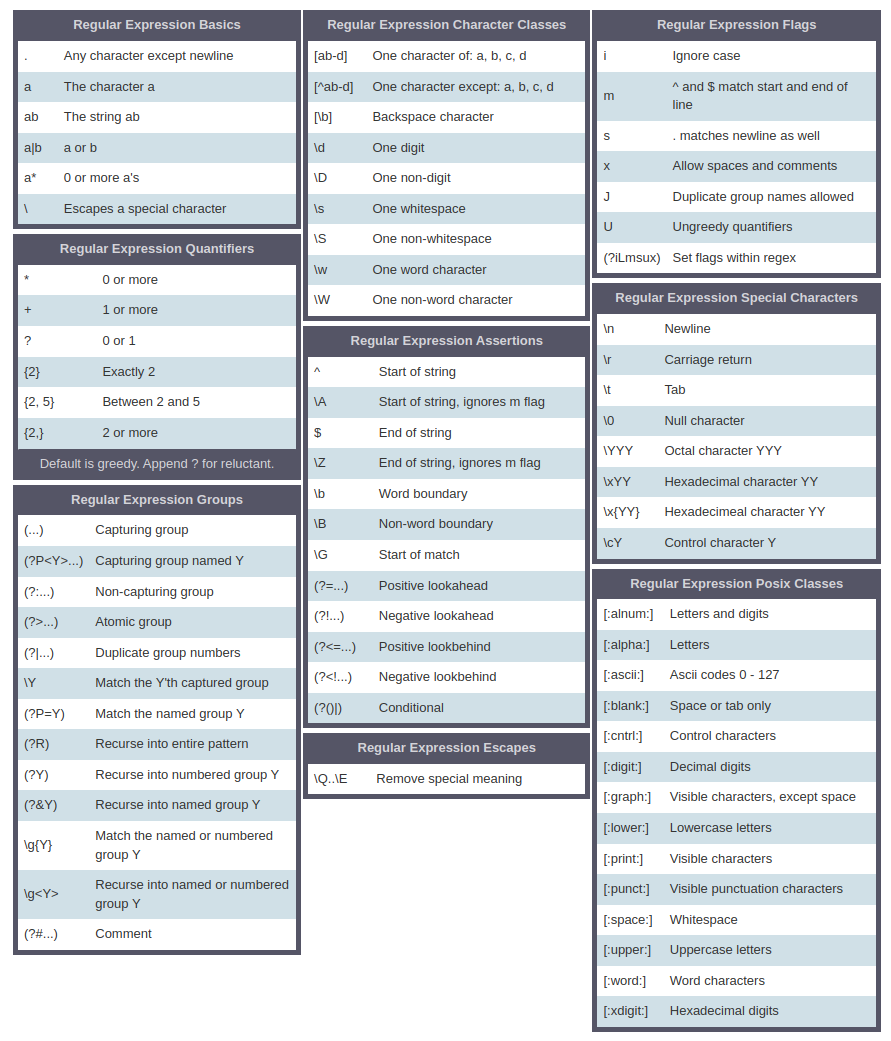
\includegraphics[width=\textwidth]{images/pcre.png}
\end{center}

测试正则表达式的网站:\href{https://www.debuggex.com/?flavor=pcre#cheatsheet}{DebuggexBeta}


\chapter{SQLite的简单使用方法}


\section{在Ubuntu22.04上安装SQLite}
使用如下命令进行安装:
\begin{minted}[linenos=true,frame=single,breaklines]{console}
sudo apt install sqlite3
sudo apt install libsqlite3-dev
\end{minted}

注意,第1行命令实际上只是提供了一个终端调试界面;要想在程序中使用SQLite,必须运行第2个命令来安装相关库,然后我们的C语言代码中的“\#include <sqlite3.h>”才能找到所需文件。

为了更方便操作SQLite,可以安装下面这个工具:
\begin{minted}[linenos=true,frame=single,breaklines]{console}
sudo apt install sqlitebrowser
\end{minted}


\section{C语言中调用SQLite的方法}
一方面,在C语言程序中添加以下代码:
\begin{minted}[linenos=true,frame=single,breaklines]{c}
#include <sqlite3.h>
\end{minted}

另一方面,在CMakeLists.txt文件中添加以下代码:
\begin{minted}[linenos=true,frame=single,breaklines]{cmake}
target_link_libraries(sqlite_c_test
                      sqlite3)
\end{minted}


\section{如何在代码中执行SQL的查询命令}
因为本项目中只有对SQLite数据库的查询操作,所以就不谈论其他操作。另外,关于SQLite数据库创建、表创建、添加记录等操作,将直接使用sqlitebrowser工具来完成,程序中不处理。

这里介绍两种方法,一种是使用 sqlite3\_exec() 函数,另一种是使用 sqlite3\_prepare\_v2() 函数。下面直接列出完整代码:
\begin{minted}[linenos=true,frame=single,breaklines]{c}
// @copyright Copyright 2023 Willard Lu
//
// Use of this source code is governed by an MIT-style
// license that can be found in the LICENSE file or at
// https://opensource.org/licenses/MIT.

#include <sqlite3.h>
#include <stdio.h>

int Callback(void *, int, char **, char **);

int main() {
  sqlite3 *db;
  char *err_msg = 0;

  // 1. 打开数据库
  int rc = sqlite3_open("test1.db", &db);
  if (rc != SQLITE_OK) {
    fprintf(stderr, "Can't open database: %s\n", sqlite3_errmsg(db));
    sqlite3_close(db);
    return 1;
  }

  // 2. 执行sql命令
  char *sql = "select * from t1";

  // 使用sqlite3_exec()函数来执行sql命令
  rc = sqlite3_exec(db, sql, Callback, 0, &err_msg);
  if (rc != SQLITE_OK) {
    fprintf(stderr, "Failed to select data\n");
    fprintf(stderr, "SQL error: %s\n", err_msg);
    sqlite3_free(err_msg);
    sqlite3_close(db);
    return 1;
  }

  // 使用sqlite3_prepare_v2预编译命令来执行sql命令
  sqlite3_stmt *res;
  rc = sqlite3_prepare_v2(db, sql, -1, &res, 0);
  if (rc == SQLITE_OK) {
    sqlite3_bind_int(res, 1, 3);
  } else {
    fprintf(stderr, "Failed to prepare statement: %s\n", sqlite3_errmsg(db));
  }
  int step = 0;
  while (1) {
    step = sqlite3_step(res); // 查询一步
    if (step == SQLITE_ROW) {
      printf("%s: ", sqlite3_column_text(res, 0));
      printf("%s\n", sqlite3_column_text(res, 1));
    } else {
      break;
    }
  }

  sqlite3_finalize(res); // 销毁预编译对象
  sqlite3_close(db); // 关闭数据库
  return 0;
}

// 回调函数
int Callback(void *NotUsed, int argc, char **argv, char **azColName) {
  NotUsed = 0;
  for (int i = 0; i < argc; i++) {
    printf("%s = %s\n", azColName[i], argv[i] ? argv[i] : "NULL");
  }
  printf("\n");
  return 0;
}
\end{minted}

从代码中可以看到,第1种方法会使用到回调函数,但这里有一个问题,就是来自数据库的数据如何更好的传递给调用程序。我们看到来自数据库的数据在回调函数中,如果想传给调用程序,似乎只能使用全局变量(回调函数不能修改参数),这显然不好。第2种方法可以妥善处理好这个问题,因此,目前使用第2种方法来获取从数据库中查询到的数据。

本章内容写得比较简单,因为这里的资料并非本项目的主线内容,详细讨论的话会需要很多时间和精力,暂无必要。这种情况在综合性项目中表现尤其突出。人的精力毕竟有限,不可能面面俱到,以后最好交由人工智能助手来整理总结归纳。


\chapter{开发日记}


\section{2023年10月}


\subsection{10月5日}
这个项目最初只是打算使用简单的判断方法来解决,但想到以后要开发其他编译器,所以先用这个微小项目来练练手。项目将按照编译器开发方法来实现,当然,本项目过于微小,大概只会用到词法分析与语法分析。

Windows系统和Linux系统在文本处理上是有些差异的,其中的换行就不相同。Windows系统中的换行实际上包含了两个字符,即$\backslash r$(回车,0xD)与$\backslash n$(换行,0xA),而Linux系统中只有$\backslash n$(换行,0xA)。我现在主要使用的是Linux系统,但为了兼顾Windows系统,可能需要在读入配置文件后,先把其中的$\backslash r\backslash n$替换成$\backslash n$,然后才做词法分析。

目前暂时只解析裸键名,引号键名以后再考虑。


\subsection{10月6日}
在绘制状态转换图时,我们看到在识别某些内容时,可以按照不同的权衡有不同的处理方式。例如在判断整数时,可以在出现非数字符号就截止,也可以规定必须要出现空格、换行符或\#才截止,两种方式一个宽松,一个严格,各有各的好处与不足。前一种方式对TOML的书写格式比较宽松,但也因为过于宽松可能导致混乱,并增加后期处理的负担。后一种方式要求严格,书写时会有更多约束,但可以减少后期处理的工作量。这里说的后期处理主要是指语法分析阶段。


\subsubsection{10月7日}
随着状态转移图绘制的深入,会让人感到越来越繁琐,或许应该创建一个专门的工具来绘制,并且在绘制完成后自动转换成相应表格直接供词法分析器调用。这个工具的原理并不复杂,麻烦的是图形操作方面的支持问题,这将涉及到图形库方面,这是一个老话题了,先放一放。


\subsection{10月12日}
绘制状态转换图时,我曾经想到对于不合法的符号要如何在图中去处理,这是一种流程图的思维习惯。实际上,在状态转换图中并不需要显式指明如何处理不合法的符号,而是已经暗含了处理方式。合法的符号串可以从状态转换图的开始(start)处走到某一个终点,不合法的符号是没有路径的,在程序处理上会自动跳到错误处理模块,通常会向用户报告某行某列出现词法错误。通常情况下,每发现一个错误就退出程序并报告此错误,也可以把每一行视为一个单元,全部扫描后统一报告。全部扫描的方式还有一些细节问题需要考虑,并非简单的逐行处理就可以。

在把状态转换图映射为状态转换表时,需要把使用到的符号、状态都列出来,这项工作的繁琐程度会随着语言的复杂程度的增加而增加。对于本项目,即使只是简化版的,其状态转换图已经有些繁琐。


\section{2023年11月}


\subsection{11月13日}
在绘制状态转换图时,对于各个状态的编号,一开始我会习惯性的从1开始顺序编写。这样做对于后面的修改并不方便,因为每次修改中间的编号都要对后续的编号重新编写。因此,现在改为使用分段编号,例如注释是100开头,祼键使用200开头。这种方法就需要在状态转换表中增加一列参数来标明编号,以取代原来隐含的自然顺序编号。在实际的程序处理中,会多出一些用于判断编号的代码,虽然会增加一点开销,但有利于设计。

原本我打算在LibreOffice Draw中用一张图来完整描绘状态转换图,但发现这张图越来越大,不利于观看,因此将其拆分为各段,并使用LaTeX的tikz宏包来绘制。虽然也可以在LibreOffice Draw中分页绘制,但为了方便本记录的查阅,就还是放在LaTeX中吧。


\subsection{11月16日}
原来的状态转换图中,无意中把数组用词法分析的形式画上去了,这实际上是不对的,正确的情况应该只是有数组中使用的定界符,即左右中括号。


\subsection{11月18日}
当编写状态转换表时,会面临以何种方式来实现的问题。最简单的方法是把这个表直接放在程序中,使用一个数组来保存,但这样做不灵活,因为每次修改都需要重新编译程序。如果我们把这个表用CSV格式存放在外部的话,灵活性确实有了,但增加了对这个表进行解析的工作。我们不能指望存放这张表的文件中全部是文本字符,应该考虑其中可能包含非文本字符的情况,因此从更通用的角度出发,需要引入转义字符的方式来可视的实现此表的编辑。毕竟不可见的符号编辑时需要使用二进制编辑工具来处理,不直观。这里我将按照C语言中转义字符的使用规则来处理,会在程序中添加一套词法解析的代码,只不过这个词法解析代码的规则将直接写在程序中,不再以外部文件的形式存放。

至此,我们可以看到,这个小项目中出现了两个词法解析,一个用于解析TOML配置文件,一个用于解析TOML的词法规则文件。


\subsection{11月21日}
使用CSV格式来保存状态转换关系,还是存在一些符号方面的问题。通常情况下,CSV分隔数据使用的是逗号,那么如果数据中包含逗号,那就需要做转义处理,一般是使用双引号。这样做感觉还是不算用户友好,所以我计划使用SQLite这一轻量级数据库来保存状态转换表。使用SQLite自然需要增加一些开销,包括引入相关源码文件和数据库管理工具,目前看来是可以接受的。这个就是数据符号与格式符号的混淆问题。

对于状态转换表中的实际内容,并不象我们绘制的图形中那样,让人想到的是一个一个的字符判断语句,具体的处理方法是使用正则表达式的规则字符串来实现。这样做可以实现通用性。例如,我们在判断一个字符是否属于字母时,一般的C语言代码中可以使用ASCII码的数值比较来判断,但这样做实际上就把规则固化在程序中,以后做调整时需要修改程序。使用正则表达式的规则字符串的话,就把程序与具体的转换规则彻底分离,以后的规则调整不再需要修改程序重新编译了。不管是什么规则,在程序中都只是简单的与内容无关的一个判断语句。


\subsection{11月28日}
开发这个工具的目的是读取TOML配置文件,那么应该向用户提供什么形式的数据输出呢?一般而言,读入TOML配置文件后,应该生成一个字符串,其中包含了数据类型、键名与键值。但仅仅是字符串的话,对于用户来说还是有些麻烦,因为需要把字符串转换成用户程序中的数据类型,这项工作应该交由本项目来完成。因此,我们还需要在本项目中添加各种数据类型的转换函数供用户调用。当然,不管最后是什么数据类型,都需要先把配置文件中的内容读取到一个字符串中保存以供后续的调用。

读取TOML配置文件后,返回给用户数据的方式有两种。一种是由用户指定键名来决定读取对应的键值,一种是把配置文件中的数据全部读取。第1种方式下,在用户程序中已经事先明确定义了相关变量;第2种方式对于C语言这样的程序,并不能直接使用,需要一些转换。第1种方式,可以先通过读取函数把TOML配置文件的内容读入到一个字符串变量中,然后再通过相应数据类型读取函数获得指定键名的键值。第2种方式因为需要使用一些转换,目前看来在用户程序中的后续调用上会增加许多开销,故此暂时不建议使用。


\section{2023年12月}


\subsection{12月02日}
我们知道软件项目的开发周期包括需求分析、设计、开发、测试、部署和维护,一共六个阶段。虽然本项目非常小,但也是如此。软件项目的开发周期中,会使用到很多工具,目的是提高整个开发过程的自动化程度,让我们可以把更多的精力放在项目真正的核心上。实际上对于大部分的软件项目,特别是进入机器人项目、人工智能项目时,项目的核心都不是计算机编程。因此在选择开发方法、工具时,一个重要的指标就是自动化程度。

本项目的开发过程确实可以使用脚本语言来逐步实现自动化,但是因为项目过小,并不具备代表性,所以暂时不做这样的处理,等开发相对完整独立的项目时再说。


\subsection{12月03日}
对于本项目在需求分析阶段的工具,我选用了数据流图(DFD),原因大家一看就明白。另外,在绘制DFD时,我用的是draw.io工具,没有使用tikz。这是因为tikz中并没有DFD方面的专用库,需要自己手动去绘制,稍显麻烦。

以前说过词法分析对应的状态转换表,表里面的字符在具体实现时用的是正则表达式的判断字符串。这样一来,实际上就不再需要针对状态转换表的进一步解析。


\subsection{12月08日}
这两天思来想去,最后还是决定不使用SQLite数据库来保存状态转换表,因为两个原因:一是处理起来稍显麻烦;二是用户使用时需要提供相关数据库文件,实际操作并不恰当。所以,我决定把TOML的相关规则放在一个头文件中,这样虽然会多增加一个文件,但却少了转换的开销。当然,不好的是每次规则的调整都需要重新编译。

在状态转换表的编写中,各种符号构成表格的横向各列,状态构成表格的纵向各行。程序运行时必须从第一个状态开始,把配置文件中传入的字符与横向各列的字符规定进行比较,如果不符合,就跳向\textcolor{red}{下一列}再比较,找到符合的列后就跳向单元格指向的状态。如果一直没有找到符合的列,就退出词法分析,并报错,这种情况通常就是配置文件中使用了非法字符。从纵向来看,如果单元格提供的状态找不到,也会退出报错,这通常是编写转换表时的疏漏造成的。


\subsection{12月10日}
当我把状态转换表放入头文件时,出现了一个问题,那就是状态转换表的编写并不友好。因为没有表格形式的支持,所以头文件中的状态转换表的数值摆放显得零乱,不易对比观察,特别是在字符类型增多时,情况会严重到几乎难以编写。因为这些原因,我现在决定还是使用CSV文件来表示,这样可以在电子表格软件来编辑,会方便很多。使用CSV文件表示的话,需要注意的一个问题就是如何正确区分正则表达式与单元格的分隔符。

默认情况下,CSV各单元格间是用逗号来分隔,每行结束时有一个换行符($\backslash$xA)。当正则表达式中出现逗号时,CSV文件一般默认使用双引号来包裹,如果出现双引号,则用两个双引号来表示一个双引号。为此,我们需要一个解析程序来分辨CSV中的正则表达式。在使用电子表格软件编辑CSV文件时,输入逗号、双引号后,很可能会被软件自动把符号从英文的符号转换为中文的符号,虽然二者在外观上差不多,但在编码上完全不一样,这点要特别注意,我在使用LibreCalc时就出现了这种情况。

另外,因为把状态转换表放在CSV文件中,所以在把本解析程序提供给用户使用时,还需要附加此CSV文件。